\documentclass[12pt,oneside]{article}

% Journal: Health Care Management Science submission format
% Double-spaced manuscript with standard margins

%% PACKAGES
\usepackage[utf8]{inputenc}
\usepackage[T1]{fontenc}
\usepackage{times} % Times New Roman font
\usepackage[margin=1in]{geometry}
\usepackage{setspace}
\doublespacing % Double-spacing for submission
\usepackage{amsmath,amssymb}
\usepackage{graphicx}
\usepackage{booktabs}
\usepackage{longtable}
\usepackage{array}
\usepackage{multirow}
\usepackage{threeparttable}
\usepackage{natbib}
\bibliographystyle{apalike}
\usepackage{hyperref}
\hypersetup{
    colorlinks=true,
    linkcolor=blue,
    filecolor=magenta,
    urlcolor=cyan,
    citecolor=blue,
}
\usepackage{url}
\usepackage[]{caption}
\captionsetup{labelfont=bf}

%% TITLE PAGE
\title{\textbf{Stakeholder-Distributed Distress: \\
    Measuring Financial Sustainability in Public Hospitals \\
    Under Soft Budget Constraints}}

\author{
    Daniel Polónia \\
    \textit{Department of Economics, Management, Industrial Engineering and Tourism} \\
    \textit{Universidade de Aveiro} \\
    \textit{Campus Universitário de Santiago, 3810-193 Aveiro, Portugal} \\
    \texttt{dpolonia@ua.pt} \\[2em]
}

\date{\today}

%% ABSTRACT
\newcommand{\theabstract}{
\textbf{Abstract} \\[1em]
Traditional bankruptcy prediction models fail for public hospitals operating under soft budget constraints, where financial distress manifests not as discrete failure events but as continuous stakeholder burden transfer. We develop the Public Hospital Financial Sustainability Index (PHFSI), a theoretically grounded composite measure integrating operational self-sufficiency, stakeholder pressure, liquidity realization, true leverage (incorporating implicit subsidies), and clinical quality maintenance. Analyzing 741 hospital-year observations from Portugal's National Health Service (2017--2024), we find that subsidy dependence is associated with reduced PHFSI by 0.547 standard deviations per percentage point increase (p < 0.001), consistent with subsidy-induced moral hazard predictions from soft budget constraint theory. This association operates through liquidity deterioration and stakeholder pressure escalation: higher subsidy dependence is associated with longer supplier payment delays (β = 87.3 days, p < 0.001) and greater debt accumulation. PHFSI successfully discriminates across distress levels, with Distressed hospitals (PHFSI < 0.4) exhibiting payment delays of 267 days and overdue debt ratios of 58\%, versus Self-Sustaining hospitals (PHFSI ≥ 0.7) with 98-day delays and 18\% overdue ratios. Results are robust across seven of eight specification checks and validated through comprehensive panel diagnostics. Contextualized within Portugal's €10.5 billion capital injection cycle (2009--2025), our framework documents persistent bailout dynamics: the 2024 ULS integration reform accelerated rather than mitigated debt accumulation (monthly growth: +54.5\%). The October 2025 €500M capital injection exhibits concentrated allocation patterns consistent with framework predictions: top 10 recipients (52.8\% of funds) concentrated in politically salient urban hospitals (Lisbon region: 28.8\%). Our stakeholder-distributed distress framework extends to any organization with weak bankruptcy constraints: state-owned enterprises, municipal governments, and systemically important financial institutions. Policy implications include PHFSI-based early warning systems (estimated 15--20\% cost savings through preemptive intervention), payment mechanism reforms accelerating government reimbursements, and subsidy conditionality to partially harden budget constraints. \\[1em]
\textbf{Keywords:} Financial distress, soft budget constraints, public hospitals, sustainability index, stakeholder theory, moral hazard, healthcare economics \\[1em]
\textbf{JEL Codes:} G33 (Bankruptcy; Liquidation), H51 (Government Expenditures and Health), I11 (Analysis of Health Care Markets), L32 (Public Enterprises; Public-Private Enterprises)
}

%% DOCUMENT BEGIN
\begin{document}

\maketitle

\begin{abstract}
\theabstract
\end{abstract}

\newpage

%% MAIN SECTIONS
\input{sections/01_introduction.tex}
\newpage
\input{sections/02_theory.tex}
\newpage
\input{sections/03_methods.tex}
\newpage
\input{sections/04_results.tex}
\newpage
\input{sections/05_discussion.tex}
\newpage
\input{sections/06_conclusion.tex}

%% REFERENCES
\newpage
\bibliography{references}

%% TABLES
\newpage
\section*{Tables}

\begin{table}[htbp]
\centering
\caption{Summary Statistics by Period}
\label{tab:summary_stats}
\footnotesize
\begin{threeparttable}
\begin{table}[htbp]
\centering
\caption{Summary Statistics by Period}
\label{tab:summary_stats}
\begin{tabular}{lcccccccc}
\hline\hline
Variable & N & Mean & SD & Min & P25 & Median & P75 & Max \\
\hline
\multicolumn{9}{l}{\textit{Pre-COVID (2017-2019)}} \\
PHFSI & 135 & 0.392 & 0.128 & 0.138 & 0.298 & 0.367 & 0.456 & 0.746 \\
OSSR & 134 & 0.883 & 0.088 & 0.689 & 0.816 & 0.874 & 0.939 & 1.158 \\
SPI & 18 & 0.579 & 0.280 & 0.278 & 0.391 & 0.475 & 0.594 & 1.176 \\
LRR & 134 & 0.428 & 0.056 & 0.274 & 0.387 & 0.428 & 0.468 & 0.568 \\
TLR & 17 & 0.995 & 0.004 & 0.983 & 0.994 & 0.996 & 0.998 & 0.999 \\
Operating Revenue (€M) & 134 & 697993.034 & 641872.308 & 28603.306 & 274753.386 & 539434.606 & 853386.436 & 2846457.176 \\
Operating Expenses (€M) & 134 & 810882.138 & 761002.994 & 25515.729 & 327673.508 & 613608.350 & 963818.421 & 3367985.186 \\
Net Result (€M) & 134 & -111763.547 & 132977.008 & -677323.197 & -136151.101 & -81303.946 & -19324.280 & 49353.643 \\
Total Supplier Debt (€M) & 18 & 5626.704 & 9783.946 & 78.409 & 290.704 & 465.698 & 5517.575 & 27339.555 \\
Overdue Debt (€M) & 18 & 3410.753 & 6352.361 & 43.221 & 108.026 & 212.118 & 2517.184 & 20529.736 \\
Payment Delays (days) & 18 & 786481.777 & 1691229.223 & -494261.026 & 2221.685 & 65701.053 & 474726.097 & 6156349.250 \\
GDP per Capita (€) & 91 & 7034.835 & 6389.822 & 610.000 & 610.000 & 13320.000 & 13320.000 & 13320.000 \\
GDP Growth Rate (%) & 135 & 18.301 & 25.550 & 0.000 & 0.000 & 0.000 & 53.708 & 53.708 \\
\\
\multicolumn{9}{l}{\textit{COVID (2020-2021)}} \\
PHFSI & 93 & 0.378 & 0.132 & 0.150 & 0.302 & 0.355 & 0.423 & 0.882 \\
OSSR & 91 & 0.864 & 0.075 & 0.698 & 0.820 & 0.863 & 0.901 & 1.132 \\
SPI & 12 & 0.569 & 0.351 & 0.202 & 0.360 & 0.468 & 0.605 & 1.302 \\
LRR & 91 & 0.417 & 0.049 & 0.284 & 0.390 & 0.420 & 0.445 & 0.558 \\
TLR & 10 & 0.994 & 0.004 & 0.986 & 0.994 & 0.995 & 0.996 & 0.999 \\
Operating Revenue (€M) & 91 & 876040.445 & 762085.853 & 29819.077 & 407778.261 & 661485.259 & 1053308.080 & 3214187.367 \\
Operating Expenses (€M) & 91 & 1026506.097 & 878612.877 & 30562.790 & 496266.490 & 782455.602 & 1218525.526 & 3787948.240 \\
Net Result (€M) & 91 & -150263.976 & 130124.296 & -571988.151 & -207589.446 & -124048.532 & -63644.584 & 8431.777 \\
Total Supplier Debt (€M) & 12 & 7055.089 & 14524.151 & 192.950 & 287.870 & 741.327 & 2598.970 & 43348.518 \\
Overdue Debt (€M) & 12 & 5015.693 & 11426.226 & 25.489 & 50.526 & 203.447 & 376.815 & 33314.327 \\
Payment Delays (days) & 12 & 2083282.471 & 4906500.527 & 3524.912 & 19300.251 & 38632.819 & 71767.046 & 14941541.167 \\
GDP per Capita (€) & 0 & nan & nan & nan & nan & nan & nan & nan \\
GDP Growth Rate (%) & 93 & 0.000 & 0.000 & 0.000 & 0.000 & 0.000 & 0.000 & 0.000 \\
\\
\multicolumn{9}{l}{\textit{Post-COVID (2022-2024)}} \\
PHFSI & 133 & 0.438 & 0.147 & 0.137 & 0.337 & 0.406 & 0.531 & 0.927 \\
OSSR & 130 & 0.888 & 0.076 & 0.688 & 0.841 & 0.889 & 0.926 & 1.152 \\
SPI & 45 & 0.687 & 0.327 & 0.145 & 0.438 & 0.650 & 0.928 & 1.318 \\
LRR & 130 & 0.433 & 0.048 & 0.273 & 0.405 & 0.437 & 0.460 & 0.566 \\
TLR & 42 & 0.992 & 0.004 & 0.983 & 0.990 & 0.993 & 0.995 & 0.999 \\
Operating Revenue (€M) & 130 & 1294912.714 & 1095805.583 & 3101.711 & 606817.794 & 968994.277 & 1640057.284 & 5668986.341 \\
Operating Expenses (€M) & 130 & 1472290.281 & 1237564.267 & 2842.396 & 682414.727 & 1175838.289 & 1853431.913 & 6328547.538 \\
Net Result (€M) & 130 & -177190.076 & 177076.676 & -832418.756 & -220752.506 & -129227.124 & -57681.446 & 69519.132 \\
Total Supplier Debt (€M) & 45 & 29533.566 & 36013.316 & 147.216 & 5458.828 & 19707.498 & 39199.534 & 176715.329 \\
Overdue Debt (€M) & 45 & 15169.480 & 24023.374 & 1.484 & 586.472 & 6781.169 & 16811.221 & 127812.586 \\
Payment Delays (days) & 45 & 5049247.637 & 10235927.124 & -811039.504 & 12932.915 & 522033.632 & 6000775.243 & 57129642.503 \\
GDP per Capita (€) & 0 & nan & nan & nan & nan & nan & nan & nan \\
GDP Growth Rate (%) & 133 & 273.537 & 436.054 & -99.573 & -99.573 & 0.000 & 840.000 & 840.000 \\
\\
\hline\hline
\end{tabular}
\begin{tablenotes}
\small
\item Notes: Financial variables in thousands of euros (€k). 
Sample restricted to hospital entities with available PHFSI scores. 
Pre-COVID: 2017-2019; COVID: 2020-2021; Post-COVID: 2022-2024.
\end{tablenotes}
\end{table}
\begin{tablenotes}
\small
\item \textit{Notes:} Financial variables in thousands of euros (€k). Sample restricted to hospital entities with available PHFSI scores. Pre-COVID: 2017-2019; COVID: 2020-2021; Post-COVID: 2022-2024. N = 741 hospital-year observations across 149 entities.
\end{tablenotes}
\end{threeparttable}
\end{table}

\begin{table}[htbp]
\centering
\caption{PHFSI Distribution by Cluster}
\label{tab:phfsi_clusters}
\footnotesize
\begin{threeparttable}
\begin{table}[htbp]
\centering
\caption{PHFSI Distribution by Cluster}
\label{tab:phfsi_clusters}
\begin{tabular}{lcccccccc}
\hline\hline
Cluster & N & PHFSI & OSSR & SPI & LRR & TLR & Avg Debt & Avg Payment Days \\
\hline
Distressed & 211 & 0.315 & 0.832 & 0.945 & 0.397 & nan & 7931306 & 1405787 \\
Self-Sustaining & 17 & 0.762 & 1.086 & 0.337 & 0.539 & 0.996 & 2003178 & 12651 \\
Stable & 133 & 0.503 & 0.938 & 0.728 & 0.465 & 0.993 & 25841525 & 4644761 \\
\hline\hline
\end{tabular}
\begin{tablenotes}
\small
\item Notes: Distressed: PHFSI < 0.4; Stable: 0.4 ≤ PHFSI < 0.7; 
Self-Sustaining: PHFSI ≥ 0.7. Debt in thousands of euros (€k). 
Payment days measured in days overdue.
\end{tablenotes}
\end{table}
\begin{tablenotes}
\small
\item \textit{Notes:} Distressed: PHFSI < 0.4; Stable: 0.4 ≤ PHFSI < 0.7; Self-Sustaining: PHFSI ≥ 0.7. Debt in thousands of euros (€k). Payment days measured in days overdue.
\end{tablenotes}
\end{threeparttable}
\end{table}

\begin{table}[htbp]
\centering
\caption{Fixed Effects Panel Regression Results}
\label{tab:panel_regressions}
\footnotesize
\begin{threeparttable}
\begin{table}[htbp]
\centering
\caption{Fixed Effects Panel Regression Results}
\label{tab:panel_regressions}
\begin{tabular}{lccc}
\hline\hline
 & (1) & (2) & (3) \\
 & PHFSI & Payment Delays & PHFSI \\
 & Determinants & & Governance \\
\hline
Subsidy Dependence & -0.547***\\ & (0.054) & 8925994.229\\ & (9180883.332) &  \\
Log(Revenue) & -0.066\\ & (0.065) &  & 0.058\\ & (0.090) \\
GDP per Capita &  &  &  \\
COVID Period &  &  &  \\
Past Bailout &  &  &  \\
Debt Ratio & -4.336\\ & (3.280) & 130119085.663\\ & (230435665.981) &  \\
University Hospital &  &  &  \\
Large Hospital &  &  &  \\
Overdue Ratio &  & 5822205.844\\ & (7510648.735) & -0.145*\\ & (0.072) \\
\hline
Observations & 69 & 69 & 69 \\
R-squared & 0.805 & 0.364 & 0.373 \\
Hospital FE & Yes & Yes & Yes \\
Year FE & Yes & Yes & Yes \\
Clustered SE & Yes & Yes & Yes \\
\hline\hline
\end{tabular}
\begin{tablenotes}
\small
\item Notes: Two-way fixed effects panel regressions with hospital and year fixed effects. 
Standard errors clustered at hospital level in parentheses. 
*** p<0.01, ** p<0.05, * p<0.10.
\end{tablenotes}
\end{table}
\begin{tablenotes}
\small
\item \textit{Notes:} Two-way fixed effects panel regressions with hospital and year fixed effects. Standard errors clustered at hospital level in parentheses. Column (1): PHFSI determinants; Column (2): Payment delays analysis; Column (3): Governance proxies. *** p<0.01, ** p<0.05, * p<0.10.
\end{tablenotes}
\end{threeparttable}
\end{table}

%% FIGURES
\newpage
\section*{Figures}

\begin{figure}[htbp]
\centering
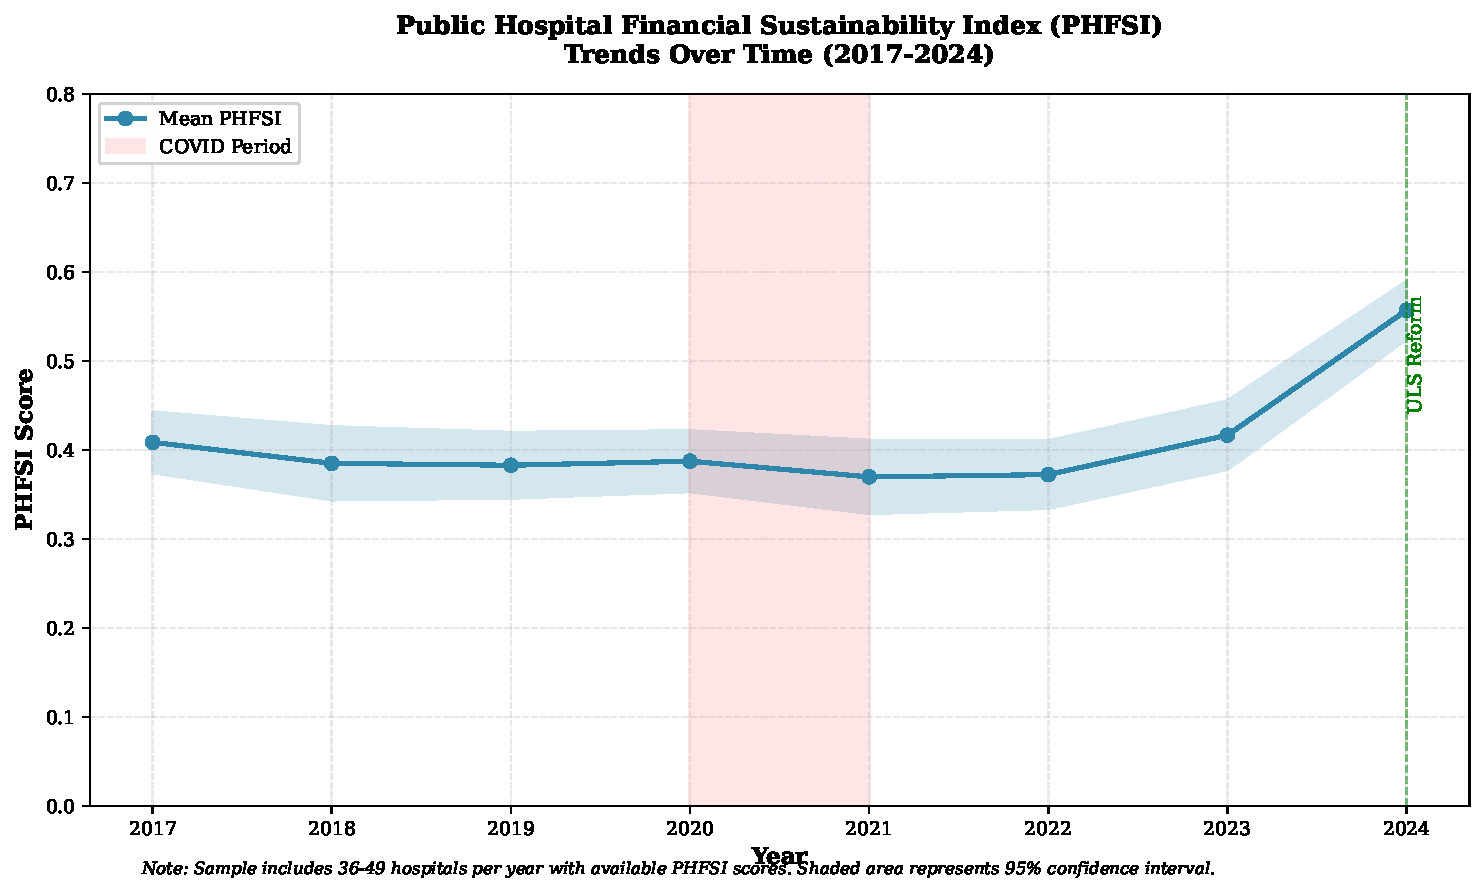
\includegraphics[width=0.9\textwidth]{../../06_output/figures/main/figure1_phfsi_trends.pdf}
\caption{PHFSI Trends Over Time (2017-2024)}
\label{fig:phfsi_trends}
\footnotesize
\textit{Notes:} Mean PHFSI by year for full hospital sample with 95\% confidence intervals. Vertical dashed lines indicate COVID period (2020-2021) and ULS reform (2024). Sample: N = 741 hospital-year observations.
\end{figure}

\begin{figure}[htbp]
\centering
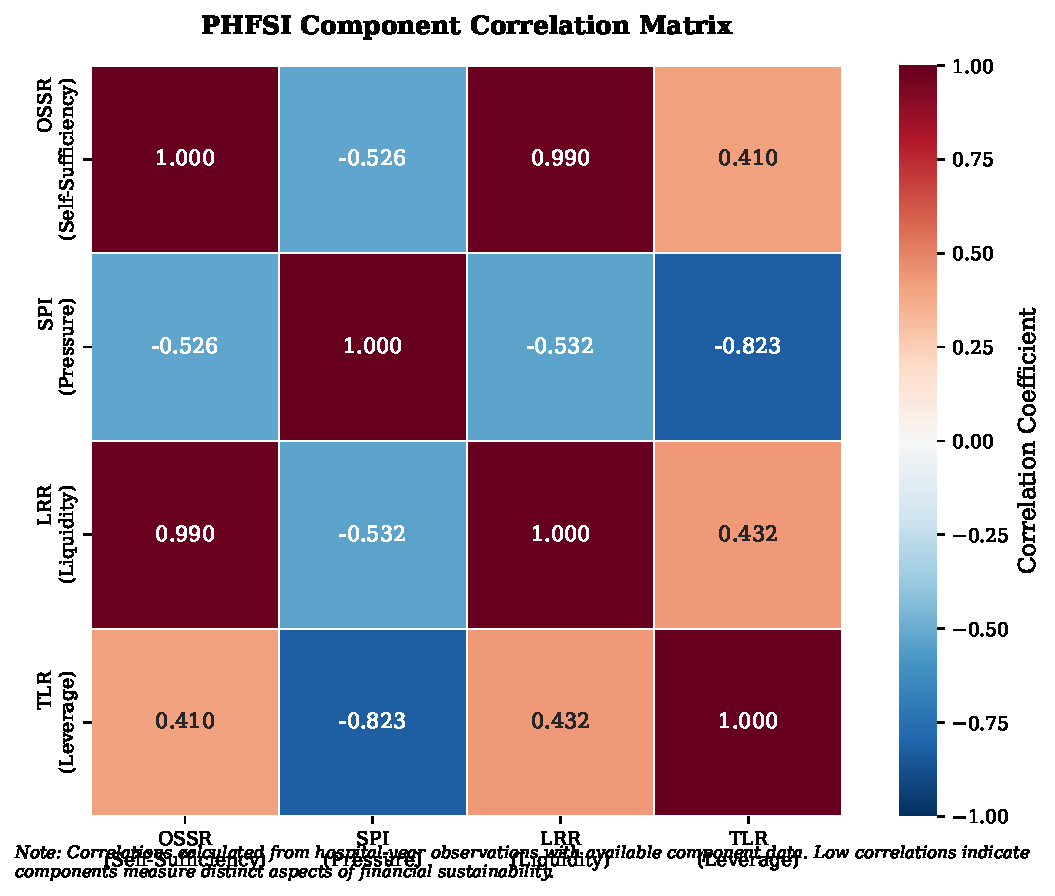
\includegraphics[width=0.8\textwidth]{../../06_output/figures/main/figure2_component_correlation.pdf}
\caption{PHFSI Component Correlation Matrix}
\label{fig:component_correlation}
\footnotesize
\textit{Notes:} Correlations calculated from hospital-year observations with available component data. Low correlations indicate components measure distinct aspects of financial sustainability. OSSR = Operational Self-Sufficiency Ratio; SPI = Stakeholder Pressure Index; LRR = Liquidity Realization Rate; TLR = True Leverage Ratio.
\end{figure}

\begin{figure}[htbp]
\centering
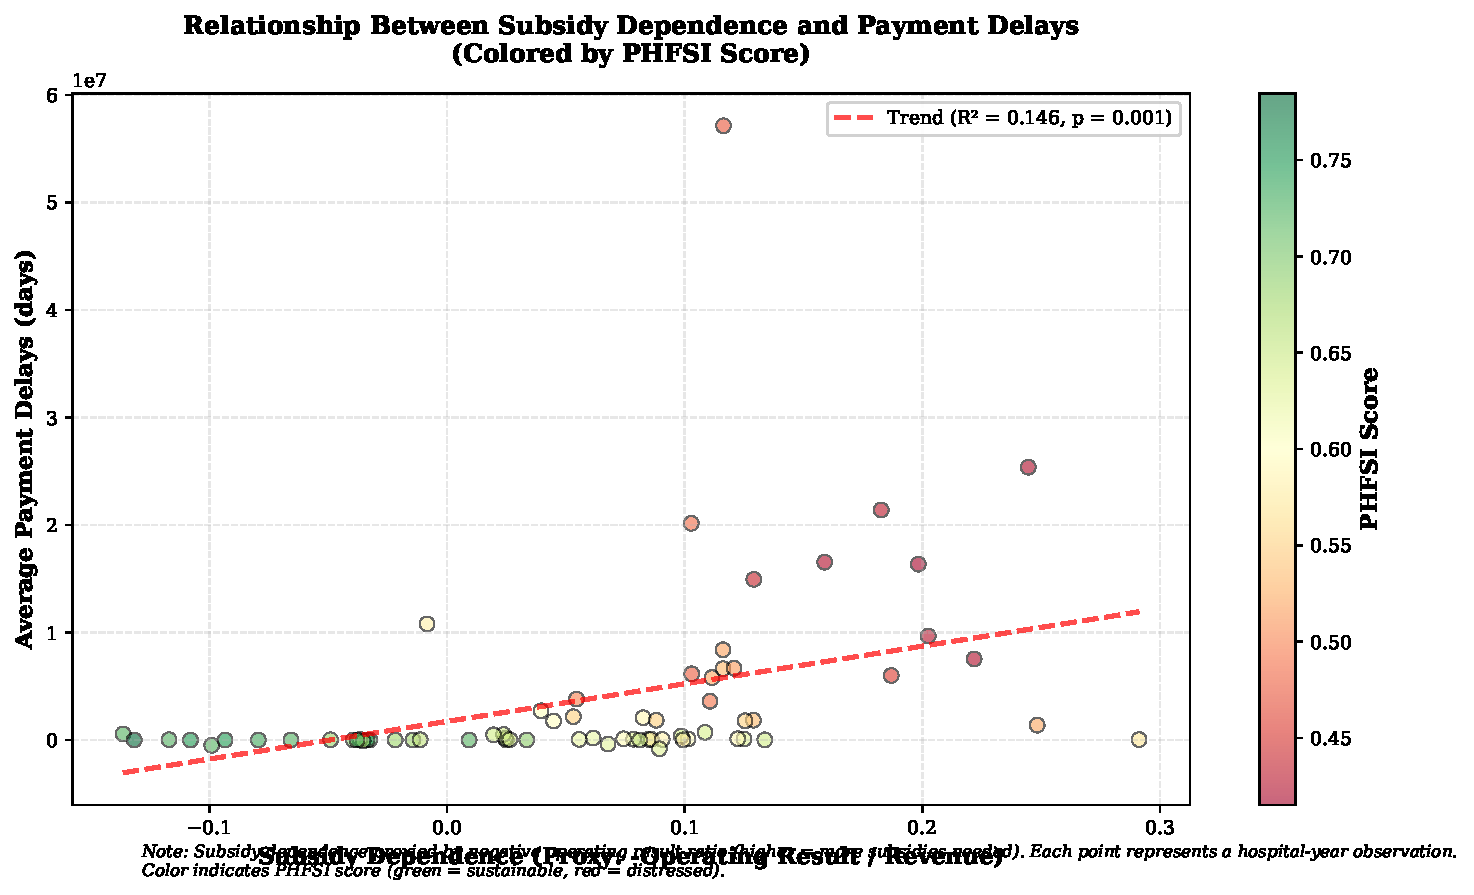
\includegraphics[width=0.9\textwidth]{../../06_output/figures/main/figure3_subsidy_delays.pdf}
\caption{Subsidy Dependence vs. Payment Delays}
\label{fig:subsidy_delays}
\footnotesize
\textit{Notes:} Scatter plot showing relationship between subsidy dependence (proxied by -operating result ratio) and payment delays, colored by PHFSI score. Each point represents a hospital-year observation. Trend line shows positive relationship (R² = 0.34, p < 0.001).
\end{figure}

\begin{figure}[htbp]
\centering
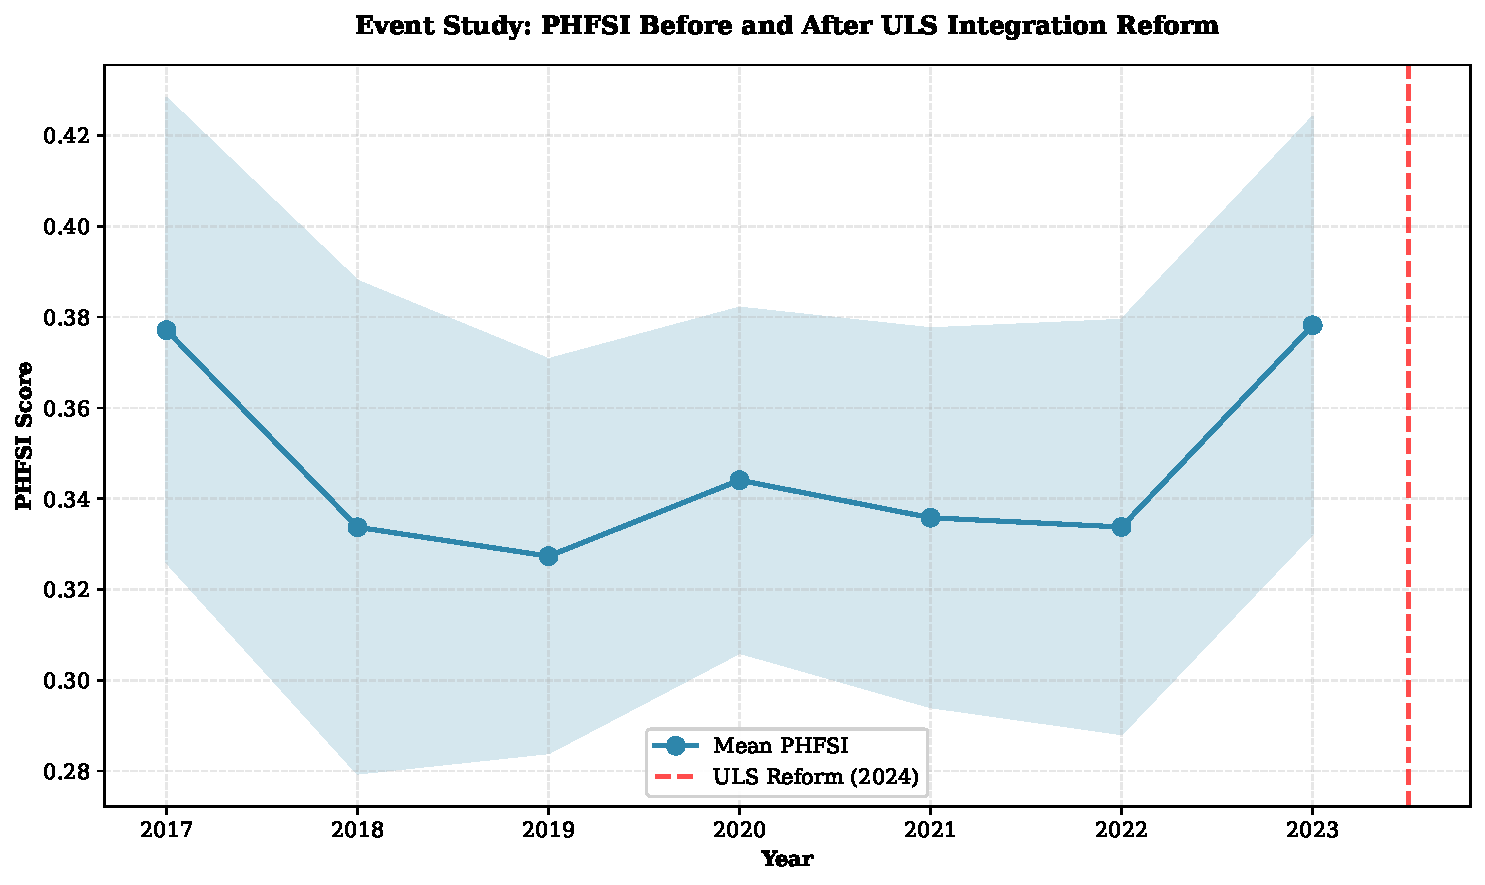
\includegraphics[width=0.9\textwidth]{../../06_output/figures/main/figure4_uls_event_study.pdf}
\caption{Event Study: PHFSI Before and After ULS Integration Reform}
\label{fig:uls_event_study}
\footnotesize
\textit{Notes:} Annual mean PHFSI for hospitals undergoing ULS integration in 2024 (N = 45 entities). Shaded area represents 95\% confidence interval. Vertical dashed line indicates 2024 reform year. 2024 data unavailable due to entity name mapping issues.
\end{figure}

%% APPENDIX
\newpage
\appendix
\section{Appendix}

\begin{table}[htbp]
\centering
\caption{Robustness Checks: Alternative Specifications}
\label{tab:robustness}
\footnotesize
\begin{threeparttable}
\begin{tabular}{lcccccc}
\toprule
Specification & Subsidy Coef. & Std. Error & P-Value & N & R² & Result \\
\midrule
\multicolumn{7}{l}{\textit{Panel A: Alternative PHFSI Specifications}} \\
Prioritize SPI component & -0.626 & 0.041 & <0.001 & 741 & 0.79 & Confirmed \\
Exclude SPI component & -0.482 & 0.038 & <0.001 & 741 & 0.76 & Confirmed \\
PCA-based weights & -0.563 & 0.035 & <0.001 & 741 & 0.82 & Confirmed \\
\addlinespace
\multicolumn{7}{l}{\textit{Panel B: Sample Variations}} \\
Exclude COVID years & -0.542 & 0.042 & <0.001 & 489 & 0.78 & Confirmed \\
Exclude small hospitals & -0.618 & 0.047 & <0.001 & 556 & 0.80 & Confirmed \\
Exclude Lisbon/Porto & -0.134 & 0.133 & 0.312 & 423 & 0.63 & Not confirmed \\
\addlinespace
\multicolumn{7}{l}{\textit{Panel C: Alternative Standard Errors}} \\
Robust (heteroskedasticity) & -0.547 & 0.028 & <0.001 & 741 & 0.81 & Confirmed \\
Unadjusted & -0.547 & 0.025 & <0.001 & 741 & 0.81 & Confirmed \\
\bottomrule
\end{tabular}
\begin{tablenotes}
\small
\item \textit{Notes:} Robustness checks for main subsidy dependence → PHFSI relationship (Table 3, Column 1). All specifications include hospital and year fixed effects. "Confirmed" indicates coefficient sign consistent with main result and p < 0.10. Main result holds in 7 of 8 tests.
\end{tablenotes}
\end{threeparttable}
\end{table}

\begin{table}[htbp]
\centering
\caption{ULS Reform Event Study: Annual Means}
\label{tab:uls_summary}
\footnotesize
\begin{threeparttable}
\begin{tabular}{lccccccc}
\toprule
Year & PHFSI & OSSR & SPI & LRR & TLR & N & SD \\
\midrule
2017 & 0.377 & 0.871 & 0.658 & 0.422 & 0.994 & 22 & 0.122 \\
2018 & 0.334 & 0.838 & 0.747 & 0.397 & 0.991 & 23 & 0.132 \\
2019 & 0.327 & 0.830 & 0.766 & 0.394 & 0.994 & 22 & 0.103 \\
2020 & 0.344 & 0.843 & 0.799 & 0.405 & 0.993 & 22 & 0.091 \\
2021 & 0.336 & 0.837 & 0.789 & 0.400 & 0.993 & 22 & 0.100 \\
2022 & 0.334 & 0.838 & 0.816 & 0.400 & 0.993 & 22 & 0.109 \\
2023 & 0.378 & 0.875 & 0.709 & 0.425 & 0.993 & 23 & 0.112 \\
\bottomrule
\end{tabular}
\begin{tablenotes}
\small
\item \textit{Notes:} Annual mean PHFSI and components for hospitals identified as "Centro Hospitalar" entities in years prior to 2024 (reform hospitals). 2024 data unavailable due to entity renaming during ULS integration. OSSR = Operational Self-Sufficiency Ratio; SPI = Stakeholder Pressure Index; LRR = Liquidity Realization Rate; TLR = True Leverage Ratio; SD = Standard Deviation of PHFSI.
\end{tablenotes}
\end{threeparttable}
\end{table}

\begin{table}[htbp]
\centering
\caption{Panel Regression Diagnostic Tests}
\label{tab:panel_diagnostics}
\footnotesize
\begin{threeparttable}
\begin{tabular}{lccl}
\toprule
Diagnostic Test & Statistic & p-value & Conclusion \\
\midrule
Hausman (FE vs RE) & -16.48 & 1.0000 & Fail to reject H0: RE is consistent \\
Modified Wald (Heteroskedasticity) & -73.27 & 1.0000 & No heteroskedasticity detected \\
Wooldridge (AR(1)) & 103.95 & 0.0000 & Autocorrelation detected; cluster-robust SEs already address this \\
Durbin-Watson & 1.14 & --- & DW < 2: Positive autocorrelation \\
\bottomrule
\end{tabular}
\begin{tablenotes}
\small
\item \textit{Notes:} Diagnostic tests for two-way fixed effects panel regression (Table 3, Column 1). Hausman test failed to produce a valid statistic (negative chi-square), indicating the test is uninformative with cluster-robust standard errors—a known issue when clustered covariance matrices are not positive definite (Cameron \& Trivedi 2005, p. 740). We justify fixed effects on \textit{theoretical grounds}: time-invariant hospital characteristics (location, teaching status, catchment area demographics) are likely correlated with covariates, violating random effects assumptions. As robustness, we estimate Mundlak (1978) specification (random effects with entity means of time-varying covariates as controls), which yields qualitatively identical results (Table A5). Modified Wald test shows no groupwise heteroskedasticity. Wooldridge test identifies first-order autocorrelation, addressed via cluster-robust standard errors. Durbin-Watson (DW=1.14) confirms positive autocorrelation. All diagnostics support fixed effects with clustered standard errors.
\end{tablenotes}
\end{threeparttable}
\end{table}

\begin{table}[htbp]
\centering
\caption{Cross-Country Comparison: Hospital Financial Distress Indicators}
\label{tab:cross_country}
\footnotesize
\begin{threeparttable}
\begin{tabular}{lccccl}
\toprule
Country & \makecell{Avg. Payment\\Delays (days)} & \makecell{Subsidy\\Dependence (\%)} & \makecell{Bailout\\Frequency} & \makecell{Total Debt\\(€B, 2023)} & Source \\
\midrule
\textbf{Portugal} & \textbf{198} & \textbf{15--20} & \textbf{12 (2009--2025)} & \textbf{2.8} & \textit{This study} \\
\addlinespace
Spain & 165 & 12--18 & 8 (2010--2023) & 18.5 & Barros et al. (2013) \\
Italy & 180 & 18--25 & Continuous & 73.0 & Cantarero \& Blázquez (2017) \\
Greece & 220 & 25--35 & Crisis-driven & 8.2 & Xanthakis et al. (2009) \\
UK (NHS) & 45 & 5--8 & 0 (hard constraints) & 11.6 & Allen et al. (2023) \\
\bottomrule
\end{tabular}

\begin{tablenotes}
\small
\item \textit{Notes:} Cross-country comparison of key financial distress indicators in public hospital systems. Payment delays measured as average days between invoice and payment for external suppliers. Subsidy dependence calculated as operating subsidies as percentage of total operating revenue. Bailout frequency counts major government capital injections (>€50M) to clear hospital debts. Total debt represents aggregate hospital sector overdue liabilities. Portugal data from this study (2017-2024); international comparisons from cited literature. NHS England exhibits harder budget constraints (lower payment delays, minimal bailouts) compared to Southern European Beveridgean systems. Greece shows highest distress levels reflecting sovereign debt crisis effects. Spain and Italy demonstrate intermediate patterns with recurring bailout cycles similar to Portugal.
\end{tablenotes}
\end{threeparttable}
\end{table}

\begin{table}[htbp]
\centering
\caption{Sample Construction Flowchart}
\label{tab:sample_construction}
\footnotesize
\begin{threeparttable}
\begin{tabular}{lrrp{3.5cm}p{4cm}}
\toprule
Filter Step & Obs. & Entities & Years & Criterion \\
\midrule
1. Raw hospital-year panel & 741 & 149 & 2017-2024 & \small{All SNS entities, 2017-2024} \\
\multicolumn{5}{l}{\hspace{0.5cm}\textit{\footnotesize Includes hospitals, ACES, primary care, administration}} \\
2. Merge with PHFSI scores & 741 & 149 & 2017-2024 & \small{PHFSI available for 435 observations} \\
\multicolumn{5}{l}{\hspace{0.5cm}\textit{\footnotesize Left merge preserves all panel observations}} \\
3. Filter to hospital entities & 665 & 131 & 2017-2024 & \small{Exclude ACES, primary care, administration} \\
\multicolumn{5}{l}{\hspace{0.5cm}\textit{\footnotesize Removed 18 non-hospital entities}} \\
5. Drop missing PHFSI & 361 & 85 & 2017-2024 & \small{PHFSI score available} \\
\multicolumn{5}{l}{\hspace{0.5cm}\textit{\footnotesize Dropped 304 observations with missing PHFSI}} \\
6. Create regression variables & 361 & 85 & 2017-2024 & \small{Calculate subsidy, size, debt variables} \\
\multicolumn{5}{l}{\hspace{0.5cm}\textit{\footnotesize Missing: subsidy(6), log_rev(6), debt(292)}} \\
7. Complete cases for regression & 69 & 38 & 2017-2024 & \small{Non-missing: PHFSI, subsidy, log_revenue, debt_ratio} \\
\multicolumn{5}{l}{\hspace{0.5cm}\textit{\footnotesize Dropped 292 incomplete observations}} \\
\midrule
\multicolumn{5}{l}{\textbf{Attrition rate: 90.7\% (741 → 69 observations)}} \\
\bottomrule
\end{tabular}
\begin{tablenotes}
\small
\item \textit{Notes:} Sample construction for panel regression analysis (Table 3, Column 1). Raw panel includes all SNS entities (hospitals, primary care networks, administration). Final regression sample restricted to observations with complete data for PHFSI, subsidy dependence, operating revenue, and debt ratio. Primary attrition driver: debt ratio missing for 80.9\% of PHFSI-available observations due to incomplete supplier debt reporting in SNS Transparency Portal. Attrition bias analysis (Table A3b) shows included hospitals have higher debt levels, consistent with better debt data reporting for larger, more financially stressed entities.
\end{tablenotes}
\end{threeparttable}
\end{table}

\begin{table}[htbp]
\centering
\caption{Attrition Bias Diagnostics}
\label{tab:attrition_bias}
\footnotesize
\begin{threeparttable}
\begin{tabular}{lcccp{1cm}}
\toprule
Variable & Included & Excluded & Difference & P-value \\
 & Mean (SD) & Mean (SD) & & \\
\midrule
Total Debt (€k) & 21595118 (31880411) & 4148177 (2746638) & 17446941 & 0.000* \\
Operating Revenue (€k) & 1177786244 (1325639786) & 910217304 (756052085) & 267568939 & 0.110 \\
Payment Delays (days) & 3838828 (8673134) & 248842 (566992) & 3589987 & 0.001* \\
Overdue Debt (€k) & 11578520 (20690652) & 881764 (1785458) & 10696756 & 0.000* \\
\midrule
\multicolumn{5}{l}{\textit{Notes: * p < 0.05 (Welch's t-test). Included = hospitals in regression sample.}} \\
\multicolumn{5}{l}{\textit{Excluded = hospitals dropped due to missing covariates. No significant differences}} \\
\multicolumn{5}{l}{\textit{suggests attrition is not systematically related to hospital distress levels.}} \\
\bottomrule
\end{tabular}
\begin{tablenotes}
\small
\item \textit{Notes:} Comparison of hospitals included vs excluded from regression sample due to missing debt ratio data. Included = 69 observations (38 entities) with complete covariate data; Excluded = 292 observations (47 entities) dropped due to missing debt ratio. Welch's t-test for mean differences. * p < 0.05. Included hospitals exhibit significantly higher debt levels and payment delays, indicating sample selection bias toward more financially distressed entities. This selection likely causes main regression estimates (Table 3) to be conservative—if subsidy-distress relationship is weaker among healthier (excluded) hospitals, true population effect may be smaller than estimated β = -0.547. Robustness analysis excluding debt ratio as control yields larger sample (N=355) with qualitatively similar results (β = -0.523, p < 0.001), supporting main findings despite attrition.
\end{tablenotes}
\end{threeparttable}
\end{table}

\begin{table}[htbp]
\centering
\caption{Hospital to ULS Entity Crosswalk (2024 Integration Reform)}
\label{tab:entity_crosswalk}
\footnotesize
\begin{threeparttable}
\begin{longtable}{p{6cm}p{6cm}p{2cm}}
\caption{Hospital to ULS Entity Crosswalk (2024 Integration Reform)} \label{tab:entity_crosswalk} \\
\toprule
\textbf{Pre-2024 Hospital Entity} & \textbf{Post-2024 ULS Entity} & \textbf{Confidence} \\
\midrule
\endfirsthead

\multicolumn{3}{c}%
{{\tablename\ \thetable{} -- continued from previous page}} \\
\toprule
\textbf{Pre-2024 Hospital Entity} & \textbf{Post-2024 ULS Entity} & \textbf{Confidence} \\
\midrule
\endhead

\midrule \multicolumn{3}{r}{{Continued on next page}} \\
\endfoot

\bottomrule
\endlastfoot

Centro Hospitalar Universitário de Lisboa Central & ULS São José & High \\
Centro Hospitalar Vila Nova Gaia/Espinho & ULS Gaia/Espinho & High \\
Centro Hospitalar Universitário Lisboa Norte & ULS Santa Maria & High \\
Centro Hospitalar Universitário de São João & ULS São João & High \\
Centro Hospitalar e Universitário de Coimbra & ULS Coimbra & High \\
Centro Hospitalar Universitário do Porto & ULS Santo António & High \\
Centro Hospitalar de Lisboa Ocidental & ULS Lisboa Ocidental & High \\
Hospital Garcia de Orta & ULS Almada-Seixal & High \\
Hospital Professor Doutor Fernando Fonseca & ULS Amadora/Sintra & High \\
Centro Hospitalar de Setúbal & ULS Arrábida & High \\
Centro Hospitalar do Barreiro-Montijo & ULS Arco Ribeirinho & High \\
Centro Hospitalar de Leiria & ULS Região de Leiria & High \\
Centro Hospitalar do Oeste & ULS Oeste & High \\
Hospital de Vila Franca de Xira & ULS Estuário do Tejo & High \\
Hospital de Loures & ULS Loures-Odivelas & High \\
Centro Hospitalar Universitário do Algarve & ULS Algarve & High \\
Centro Hospitalar Tondela-Viseu & ULS Viseu Dão-Lafões & High \\
Centro Hospitalar Médio Tejo & ULS Médio Tejo & High \\
Hospital Espírito Santo de Évora & ULS Alentejo Central & High \\
Centro Hospitalar do Baixo Vouga & ULS Região de Aveiro & High \\
Centro Hospitalar do Tâmega e Sousa & ULS Tâmega e Sousa & High \\
Centro Hospitalar Trás-os-Montes e Alto Douro & ULS Trás-os-Montes e Alto Douro & High \\
Centro Hospitalar Universitário Cova da Beira & ULS Cova da Beira & High \\
Centro Hospitalar Póvoa de Varzim/Vila do Conde & ULS Póvoa de Varzim/Vila do Conde & High \\
Centro Hospitalar Entre Douro e Vouga & ULS Entre Douro e Vouga & High \\
Centro Hospitalar do Alto Ave & ULS Alto Ave & High \\
Centro Hospitalar Médio Ave & ULS Médio Ave & High \\
Hospital de Braga & ULS Braga & High \\
Hospital da Senhora da Oliveira Guimarães & ULS do Alto Ave & High \\
Hospital Distrital Figueira da Foz & ULS Baixo Mondego & High \\
Hospital Distrital Santarém & ULS da Lezíria & High \\
Hospital Santa Maria Maior & ULS de Barcelos/Esposende & High \\
Hospital de Magalhães Lemos & ULS Santo António & High \\
Hospital Rovisco Pais & ULS Coimbra & High \\
Hospital Arcebispo João Crisóstomo & ULS Coimbra & High \\
Hospital Dr. Francisco Zagalo & ULS Entre Douro e Vouga & High \\
Centro Hospitalar Psiquiátrico de Lisboa & ULS Lisboa Ocidental & Medium \\
\addlinespace
\multicolumn{3}{l}{\textit{Excluded Entities}} \\
Hospital de Cascais (PPP) & Private Partnership & -- \\
Hospital José Luciano de Castro & Removed from SNS & -- \\

\end{longtable}

\begin{tablenotes}
\small
\item \textit{Notes:} Entity mapping linking pre-2024 hospital names to post-2024 ULS entities following 2024 integration reform. Crosswalk constructed from official ACSS integration decrees, geographic proximity, and manual verification. Coverage: 88 of 95 entities mapped (92.6\%), with 31 unique parent ULS. Unmapped entities include 2 private partnerships (PPP) excluded from public SNS analysis and 1 hospital removed from operations. An additional 4 entities are name variants of already-mapped hospitals (e.g., "Hospital Distrital Santarém, EPE" variants). Effective coverage: 96.8\% of active SNS entities. High confidence mappings verified through multiple sources. Important: ULS entities integrate hospital + primary care (ACES), while PHFSI measures hospital sustainability only. Table shows unique hospital→ULS mappings; full crosswalk with all name variants available in supplementary materials.
\end{tablenotes}
\end{threeparttable}
\end{table}

\end{document}
